% !TeX root = ../libro.tex
% !TeX encoding = utf8

\chapter{Implementación y pruebas}


\section{Optimización del código GLSL}
	Puesto que queremos que el programa renderice la escena en tiempo real, es necesario simplificar todo lo posible el código de los shaders, sobre todo del fragment shader (se va a ejecutar para cada vértice generado en el teselado). Para ello se han tenido en cuenta los siguientes hechos (FUENTE GLSL OPTIMIZATIONS):
	\begin{itemize}
		\item Evitar el uso de saltos condicionales y de bucles. En caso de ser necesario algún bucle, usar los de la forma ``for(int i=$0$; i<n; i++)'' con $n$ entero constante, para permitir el desenrollado del bucle por el compilador.
		\item Utilizar ``Swizzle'' en vez de asignar vectores componente a componente.
		\item Utilizar ``MAD'', es decir, usar siempre que sea posible la multiplicación por el inverso en vez de la división (para aquellos valores ``uniform'' o constantes) y desarrollar las expresiones como una sumatoria de productos. Por ejemplo, utilizar $a*0.5 + b*0.5$ en vez de $(a+b)/2$.
		\item Utilizar ``dot'' para agrupar varias expresiones en 1. De igual forma utilizar todo el cálculo vectorial y matricial posible para resumir las operaciones.
		\item Si una expresión es común para un mismo frame, calcularlo en la CPU y asignarlo como otro ``uniform'' para quitarle carga a la GPU, ya que se ejecutaría para cada primitiva o vértice (dependiendo de en qué shader se realize el cálculo).
	\end{itemize}
	
	Es cierto que el compilador ya realiza de manera automática algunas de estas optimizaciones, pero su puesta en práctica reduce ligeramente el tiempo de compilación.

\section{Generación de informes}

	Para medir el rendimiento de la aplicación se han medido los fotogramas generados por segundo y las primitivas que hay presentes en la escena, incluyendo las que son producto del teselado.\\
\\La medición del nº de primitivas se ha realizado mediante el uso de la estructura "query" de OpenGL, la cual se actualiza cada vez que renderiza la escena. El nº de fotogramas por segundo se ha calculado manualmente, a partir de la latencia entre fotogramas (cuando se acumula más de $1$ segundo de latencia, devuelve el nº de fps en ese segundo).\\
\\Además, para mayor comodidad se ha añadido una opción para realizar dichas mediciones de forma automática y escribir los resultados en un archivo cuyo nombre dependerá de la parametrización actual y el modo de visualización. Por defecto realiza $22$ medidas ($22$ segundos). Es ligeramente mayor que $20$ para después quitar la primera y/o última medida, ya que están influenciadas por la interacción del usuario con la interfaz.\\
\\Estas medidas son suficientes para observar si la aplicación está aprovechando correctamente los recursos para obtener una buena visualización de la superficie, ya que el objetivo es que funcione en tiempo real ofreciendo la mínima carga posible al sistema.

\section{Resultados}
	En esta sección se mostrarán los datos medidos en la aplicación para comparar las técnicas usadas. Se han seleccionado 2 superficies de las disponibles como ejemplos, ``gaussiana.in'' y ``waves.in''. Los parámetros se han elegido de manera que la visualización sea similar entre los distintos modos de renderizado, minimizando el nº de triángulos de la escena para cada modo, que es el objetivo de estudio: ofrecer un nivel de aproximación específico, maximizando el rendimiento.
		
	\begin{center}
	\begin{tabular}{ | p{2cm} | | p{2cm} | p{2cm} | p{2cm} | p{2cm} | p{2cm} | }
		\hline
		\multicolumn{6}{ | c | } {gaussiana.in}\\
		\hline
		$ $ &
		\multicolumn{5}{ | c | } {FPS}\\
		\hline
		Modo & Min & Max & Media & Mejora (fps) & Mejora ($\%$) \\
		\hline
		No tess.    & $205$ & $250$ & $231,54$ & $-$ & $-$ \\
		Normal tess.    & $253$ & $278$ & $267,63$ & $+36,09$ & $+15,58$ \\
		Improve1 & $242$ & $282$ & $266,63$ & $+35,09$ & $+15,15$ \\
		Improve2 & $\boldsymbol{255}$ & $\boldsymbol{284}$ & $\boldsymbol{273,72}$ & $\boldsymbol{+42.18}$ & $\boldsymbol{+18,21}$ \\
		\hline
		$ $ &
		\multicolumn{5}{ | c | } {Triángulos}\\
		\hline
		Modo & Min & Max & Media & Mejora (tri.) & Mejora ($\%$) \\
		\hline
		No tess.    & $20000$ & $20000$ & $20000,00$ & $-$ & $-$ \\
		Normal tess.    & $10547$ & $11802$ & $11165,5$ & $-8834,50$ & $-44,17$ \\
		Improve1 & $8267$ & $10232$ & $9100,00$ & $-10900,00$ & $-54,5$ \\
		Improve2 & $\boldsymbol{6642}$ & $\boldsymbol{10120}$ & $\boldsymbol{8212,68}$ & $\boldsymbol{-11787,31}$ & $\boldsymbol{-58,93}$ \\
		\hline
	\end{tabular}
	\end{center}
	\begin{figure}[h]
  		\centering
  		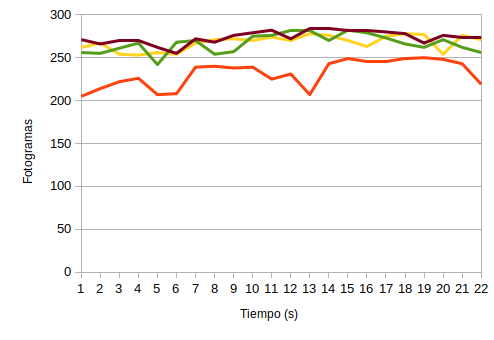
\includegraphics[width=0.435\textwidth]{performance/diagrama_gauss_fps_rec}
  		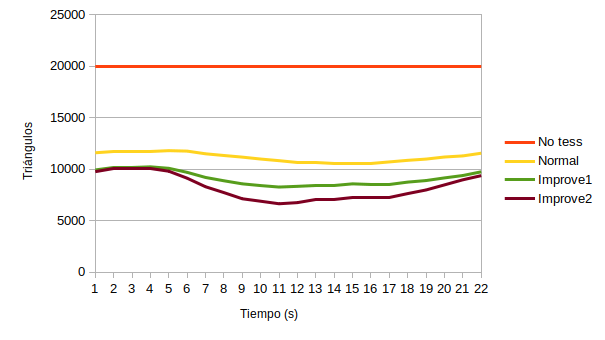
\includegraphics[width=0.555\textwidth]{performance/diagrama_gauss_triangulos}
  		\caption{Gráfica de la animación de rotación en gauss.in}
  		\label{fig:diagramas_gauss}
	\end{figure}
	
	\newpage
	\begin{center}
	\begin{tabular}{ | p{2cm} | | p{2cm} | p{2cm} | p{2cm} | p{2cm} | p{2cm} | }
		\hline
		\multicolumn{6}{ | c | } {waves.in}\\
		\hline
		$ $ &
		\multicolumn{5}{ | c | } {FPS}\\
		\hline
		Modo & Min & Max & Media & Mejora (fps) & Mejora ($\%$) \\
		\hline
		No tess.    & $21$ & $24$ & $21,81$ & $-$ & $-$ \\
		Normal tess. & $53$ & $63$ & $58,27$ & $+36,45$ & $+167,08$ \\
		Improve1 & $\boldsymbol{63}$ & $72$ & $64,68$ & $+42,86$ & $+196,45$ \\
		Improve2 & $62$ & $\boldsymbol{87}$ & $\boldsymbol{69,86}$ & $\boldsymbol{+48.04}$ & $\boldsymbol{+220,20}$ \\
		\hline
		$ $ &
		\multicolumn{5}{ | c | } {Triángulos}\\
		\hline
		Modo & Min & Max & Media & Mejora (tri.) & Mejora ($\%$) \\
		\hline
		No tess.    & $1000000$ & $1000000$ & $1000000,00$ & $-$ & $-$ \\
		Normal tess.    & $456480$ & $637537$ & $550527,77$ & $-449472,22$ & $-44,94$ \\
		Improve1 & $197244$ & $224222$ & $212327,00$ & $-787673,00$ & $-78,76$ \\
		Improve2 & $\boldsymbol{194703}$ & $\boldsymbol{223824}$ & $\boldsymbol{210390,31}$ & $\boldsymbol{-789609,68}$ & $\boldsymbol{-78,96}$ \\
		\hline
	\end{tabular}
	\end{center}
	\begin{figure}[h]
  		\centering
  		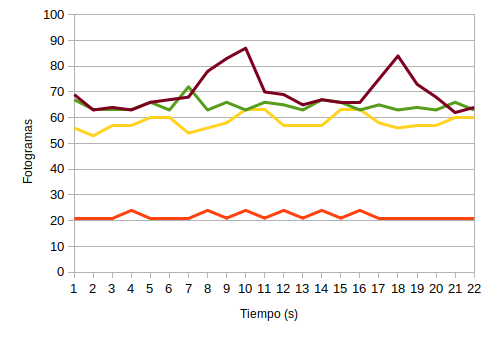
\includegraphics[width=0.435\textwidth]{performance/diagrama_waves_fps_rec}
  		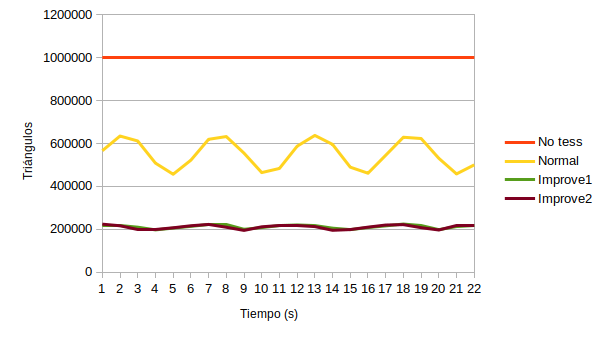
\includegraphics[width=0.555\textwidth]{performance/diagrama_waves_triangulos}
  		\caption{Gráfica de la animación de rotación en waves.in}
  		\label{fig:diagramas_waves}
	\end{figure}
	
	
	\newpage
	Las siguientes imágenes corresponden con la parametrización ``gaussiana.in'' con los distintos modos de visualización, donde para cada modo se ha buscado la configuración óptima, es decir, aquella en la que se ve visualmente bien y el nº de triángulos es mínimo. Por tanto, las $4$ imágenes debería ser exactamente iguales:
	\begin{figure}[h]
		\begin{minipage}{0.48\textwidth}
  			\centering
  			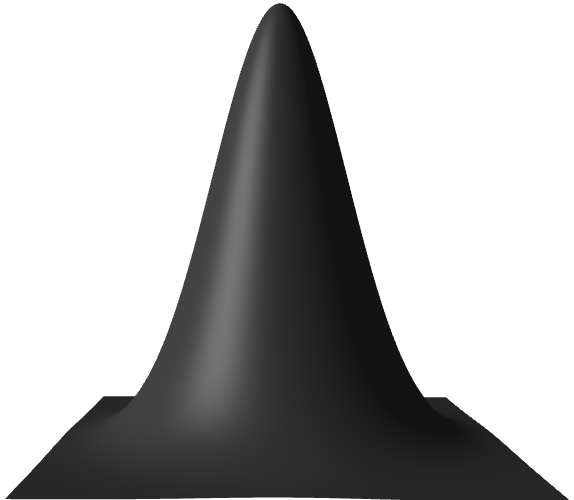
\includegraphics[width=0.9\textwidth]{performance/gauss_notess}
  			\caption{gaussiana.in sin teselar}
		\end{minipage}\hfill
		\begin{minipage}{0.48\textwidth}
  			\centering
  			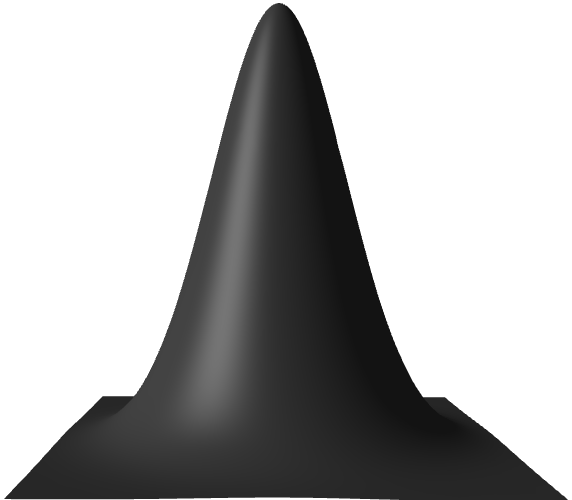
\includegraphics[width=0.9\textwidth]{performance/gauss_tessbad}
  			\caption{gaussiana.in teselado normal}
		\end{minipage}\hfill
		
		\begin{minipage}{0.48\textwidth}
  			\centering
  			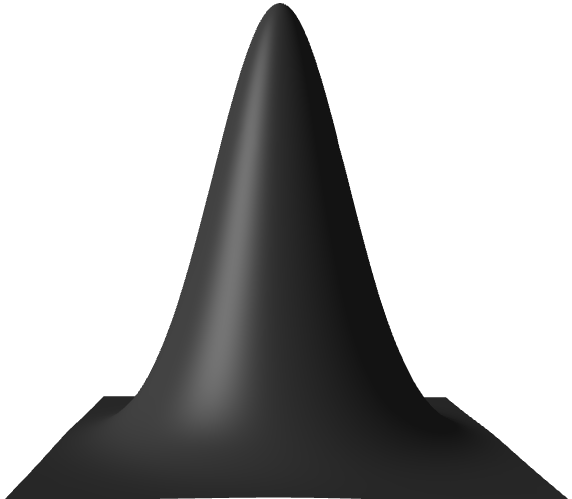
\includegraphics[width=0.9\textwidth]{performance/gauss_improve1}
  			\caption{gaussiana.in improve$1$}
		\end{minipage}\hfill
		\begin{minipage}{0.48\textwidth}
  			\centering
  			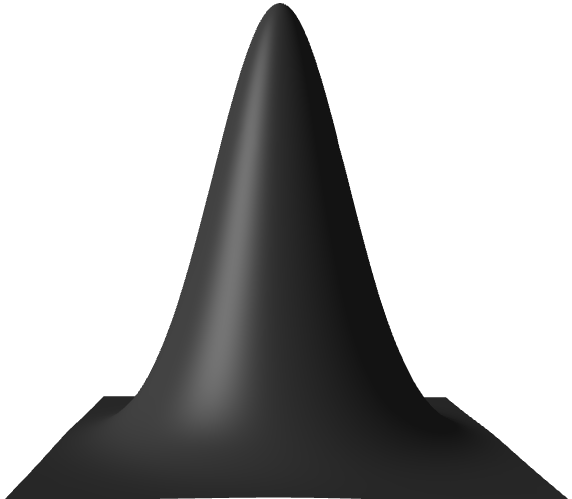
\includegraphics[width=0.9\textwidth]{performance/gauss_improve2}
  			\caption{gaussiana.in improve$2$}
		\end{minipage}\hfill
  		\label{fig:imagenes_gauss}
	\end{figure}	
	
	\newpage
	\begin{figure}[h]
		\begin{minipage}{0.48\textwidth}
  			\centering
  			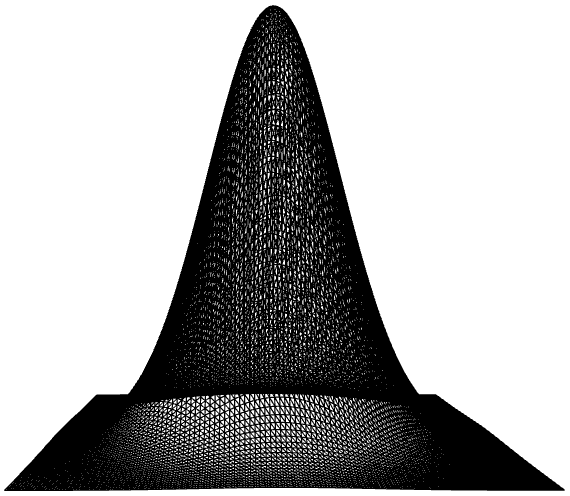
\includegraphics[width=0.9\textwidth]{performance/gauss_pol_notess}
  			\caption{gaussiana.in sin teselar}
		\end{minipage}\hfill
		\begin{minipage}{0.48\textwidth}
  			\centering
  			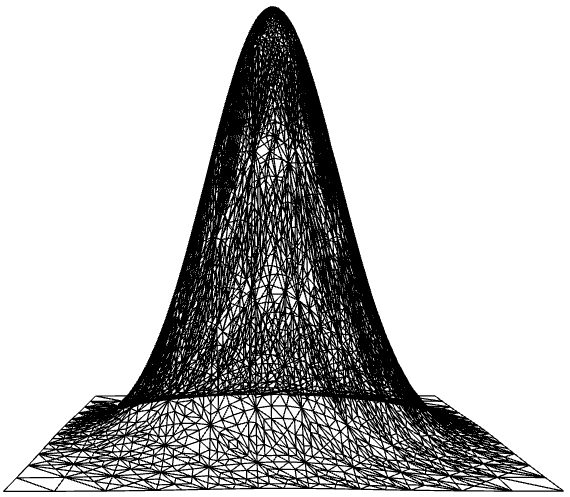
\includegraphics[width=0.9\textwidth]{performance/gauss_pol_tessbad}
  			\caption{gaussiana.in teselado normal}
		\end{minipage}\hfill
		
		\begin{minipage}{0.48\textwidth}
  			\centering
  			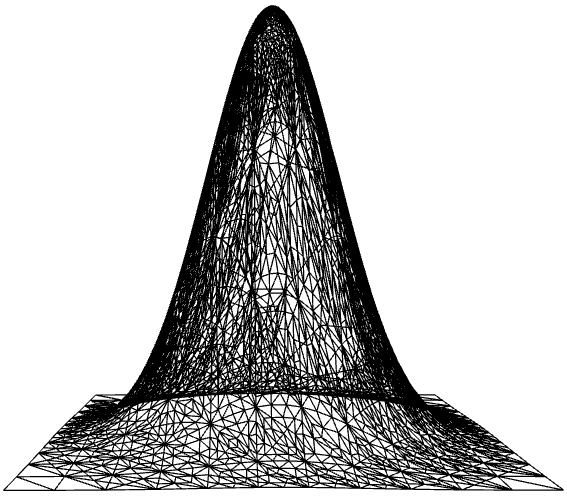
\includegraphics[width=0.9\textwidth]{performance/gauss_pol_improve1}
  			\caption{gaussiana.in improve$1$}
		\end{minipage}\hfill
		\begin{minipage}{0.48\textwidth}
  			\centering
  			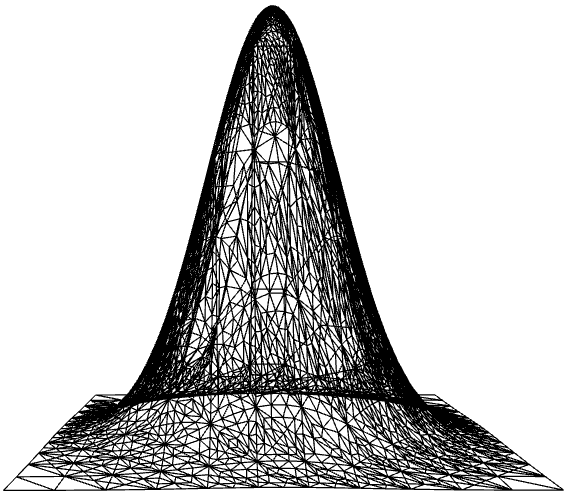
\includegraphics[width=0.9\textwidth]{performance/gauss_pol_improve2}
  			\caption{gaussiana.in improve$2$}
		\end{minipage}\hfill
  		\label{fig:imagenes_gauss_pol}
	\end{figure}	
	
	Seguidamente se muestran las imagenes correspondientes a la parametrización ``waves.in''. Sin embargo, debido a la complejidad de la superficie base (plano horizontal perturbado con un coseno), para el modo ``sin teselado'' es imposible llegar a una buena representación incluso utilizando una malla inicial de $1$ millón de triángulos, debido a la aparición de efectos ópticos, por la uniformidad de la malla inicial (parece haber más de un foco mientras que sólo hay uno).\\
	\\También es posible observar que al pasar de ``improve$1$'' a ``improve$2$'' puede aparecer algún segmento sin teselar. Se debe a que detecta que es un segmento oculto, mediante un cálculo basado en los extremos del segmento, pero como ya se comentó anteriormente esta funcionalidad está pensada para superficies específicas.
	\newpage
	\begin{figure}[h]
  		\centering
  		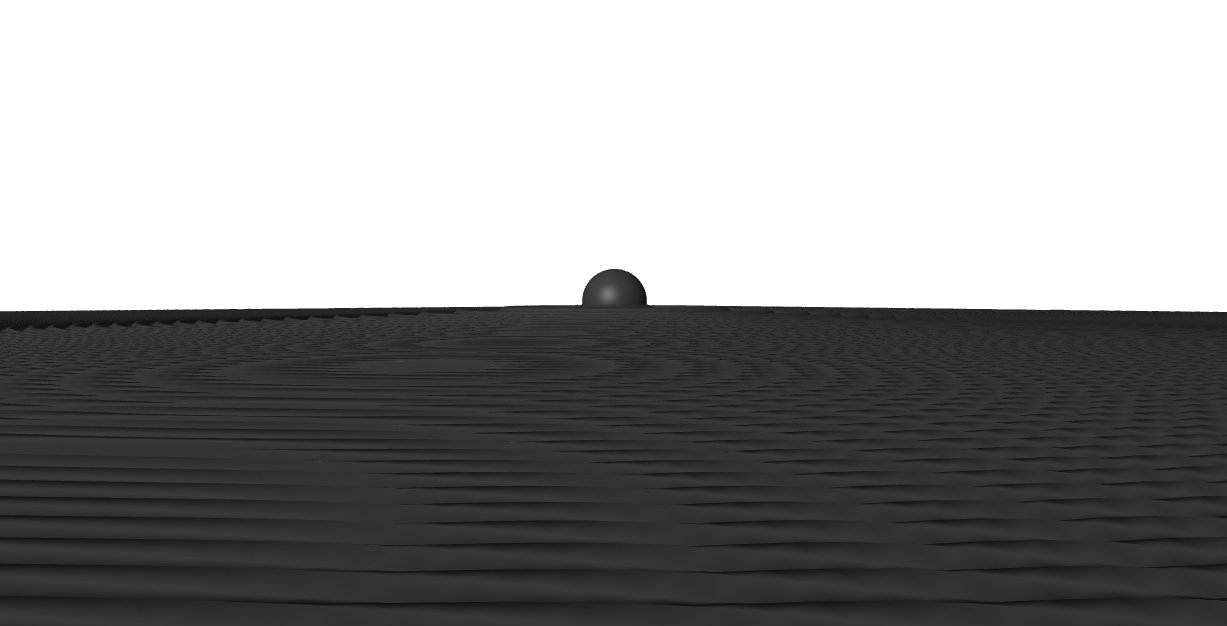
\includegraphics[width=0.9\textwidth]{performance/waves_notess}
  		\caption{waves.in sin teselar}
  		\vspace{0.5cm}
  		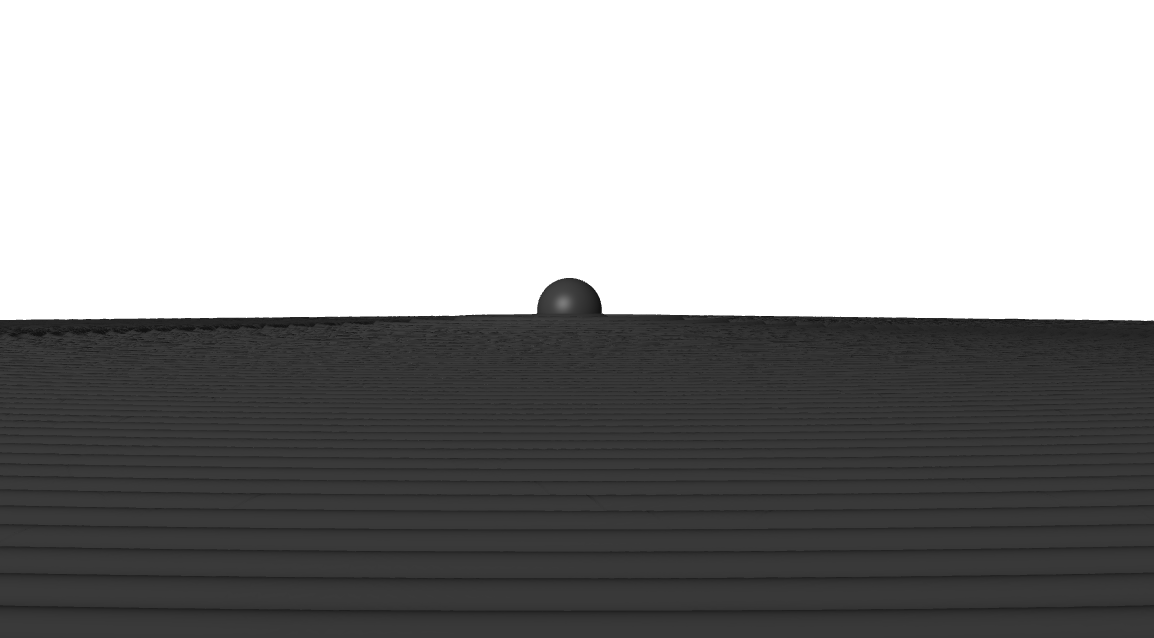
\includegraphics[width=0.9\textwidth]{performance/waves_tessbad}
  		\caption{waves.in teselado normal}
  		\vspace{0.5cm}
  		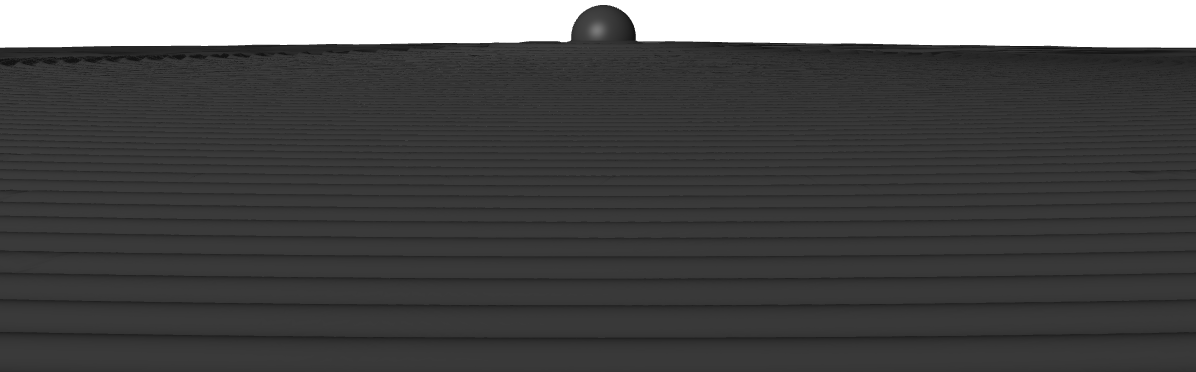
\includegraphics[width=0.9\textwidth]{performance/waves_improve1}
  		\caption{waves.in improve$1$}
  		\vspace{0.5cm}
  		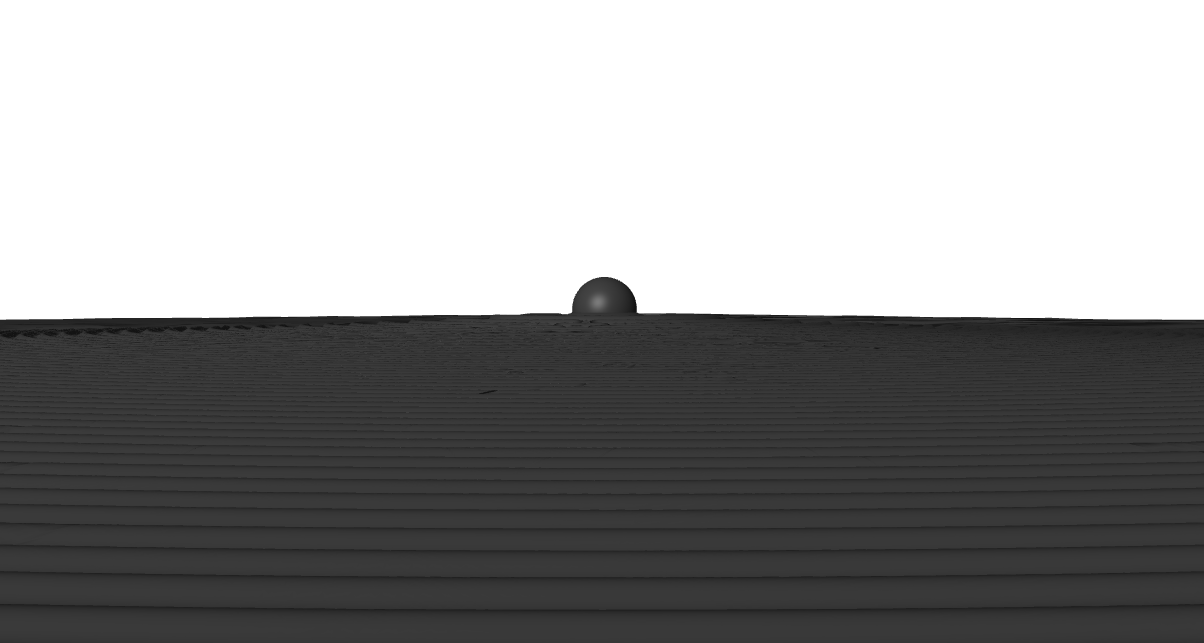
\includegraphics[width=0.9\textwidth]{performance/waves_improve2}
  		\caption{waves.in improve$2$}
  		\label{fig:imagenes_waves}
	\end{figure}	
	\begin{figure}[h]
  		\centering
  		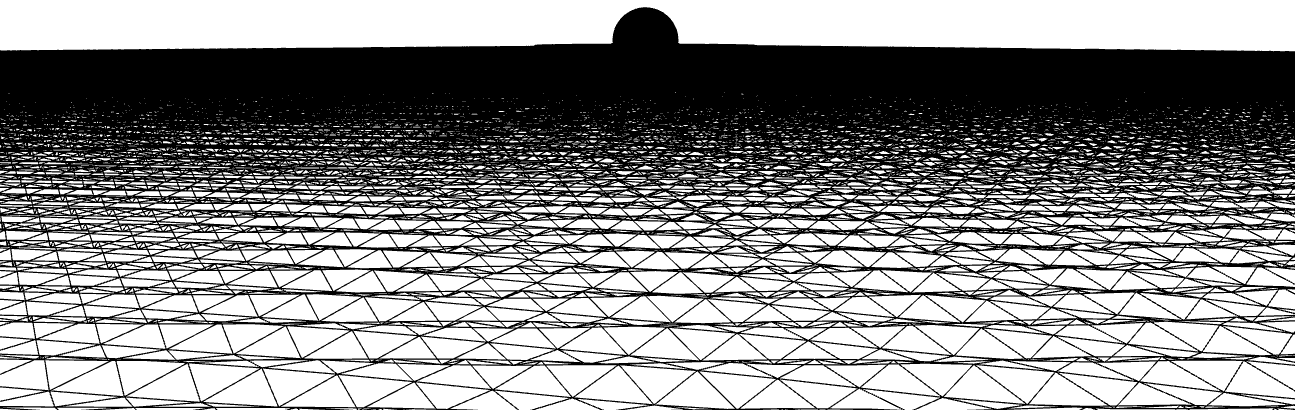
\includegraphics[width=0.9\textwidth]{performance/waves_pol_notess}
  		\caption{waves.in sin teselar}
  		\vspace{0.5cm}
  		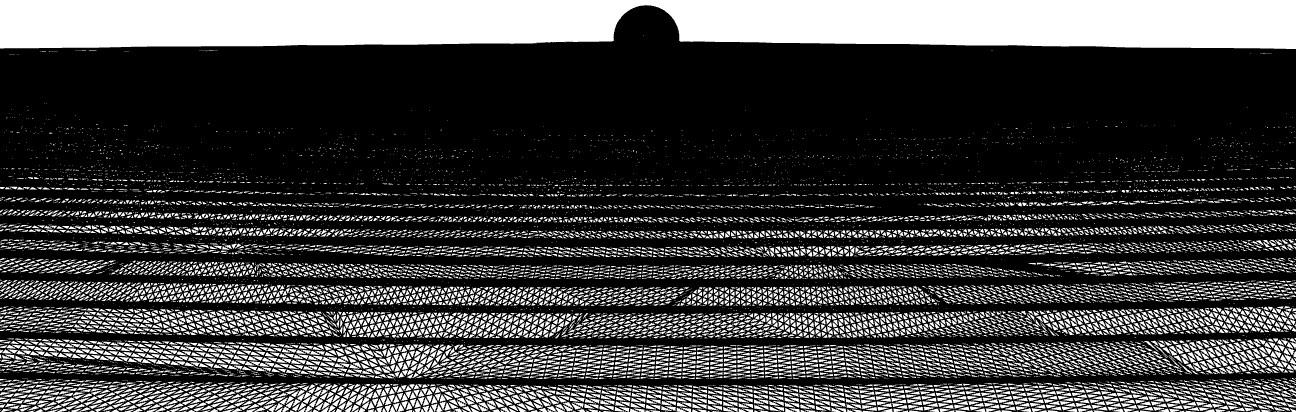
\includegraphics[width=0.9\textwidth]{performance/waves_pol_tessbad}
  		\caption{waves.in teselado normal}
  		\vspace{0.5cm}
  		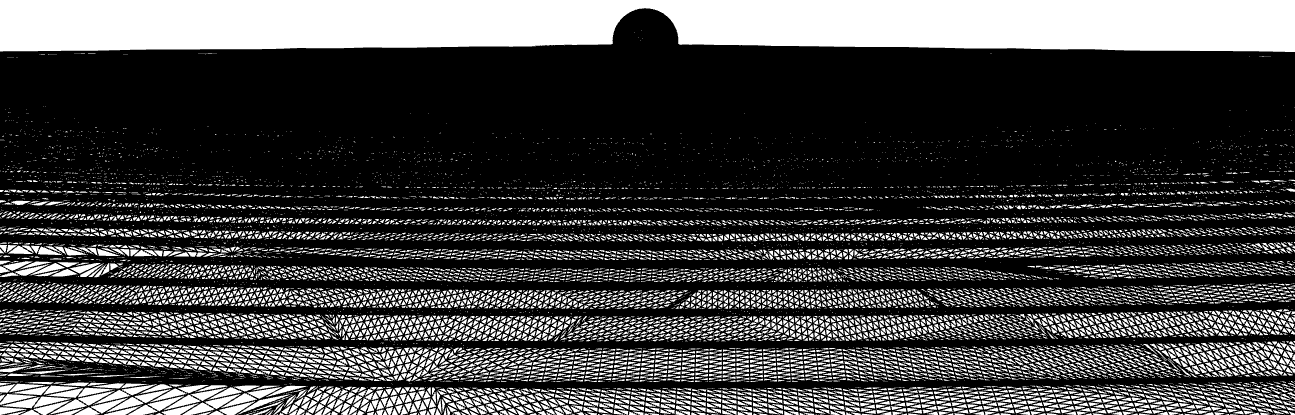
\includegraphics[width=0.9\textwidth]{performance/waves_pol_improve1}
  		\caption{waves.in improve$1$}
  		\vspace{0.5cm}
  		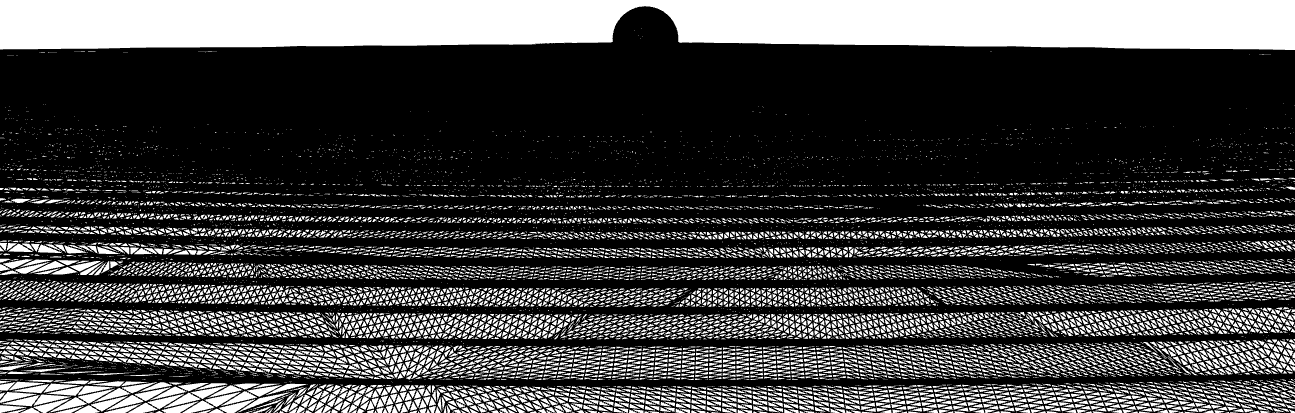
\includegraphics[width=0.9\textwidth]{performance/waves_pol_improve2}
  		\caption{waves.in improve$2$}
  		\label{fig:imagenes_waves_pol}
	\end{figure}	
	\newpage
		
		
\endinput
%------------------------------------------------------------------------------------
% FIN DEL CAPÍTULO. 
%------------------------------------------------------------------------------------
